\subsection{Nodo di controllo}

\subsubsection{Aritificial Potential Field}
Per poter utilizzare tale tipologia di controllo bisogna calcolare il \textit{goal} dinamicamente, cioè calcolare l'intersezione tra la retta e il cerchio di raggio r. Ricodiamo che le coordinate $(x_r,y_r)$ coincidono con quelle del rover. Impostando il sistema:

\begin{equation} 
\begin{cases}

    (x-x_r)^2+(y-y_r)^2=r^2
   \\
    y=mx+q 
  \end{cases} 
\end{equation}
si sostituisce la seconda equazione nella prima
\begin{equation}
(x-x_r)^2+(mx+q-y_r)^2=r^2
\end{equation}

\begin{equation}
x^2+x_r^2-2xx_r+m^2x^2+q^2+y_r^2+2mxq-2mqy_r-2mxy_r-r^2=0
\end{equation}

\begin{equation}
\underbrace{(1+m^2)}_\text{a}x^2+\underbrace{(2mq-2x_r-2my_r)}_\text{b}x+\underbrace{(x_r^2+q^2+y_r^2-2qy_r-r^2)}_\text{c}=0
\end{equation}
Definiamo $\Delta=b^2-4ac=(2mq-2x_r-2my_r)^2-4(1+m^2)(x_r^2+q^2+y_r^2-2qy_r-r^2)$. \\Se:
\begin{itemize}
    \item $\Delta>0$ si hanno due soluzioni
        \begin{equation}
        x_1=\frac{-(2mq-2x_r-2my_r)+\sqrt{2mq-2x_r-2my_r)^2-4(1+m^2)(x_r^2+q^2+y_r^2-2qy_r-r^2)}}{2(1+m^2)}
        \end{equation}
        \\
        \begin{equation}
        x_2=\frac{-(2mq-2x_r-2my_r)-\sqrt{2mq-2x_r-2my_r)^2-4(1+m^2)(x_r^2+q^2+y_r^2-2qy_r-r^2)}}{2(1+m^2)}
        \end{equation}
        Di queste due soluzioni si sceglie quella più lontana rispetto alla posizione dell'ArUco.
    \item $\Delta=0$ si ha una sola soluzione
    \begin{equation}
        x_d=\frac{-(2mq-2x_r-2my_r)}{2(1+m^2)}
        \end{equation}
    \item $\Delta<0$ non si hanno soluzioni, per cui usiamo la proiezione ortogonale tra la retta $y=mx+q$ e la retta passante per le coordinate $(x_r, y_r)$ del rover.
\end{itemize}
Il punto così ottenuto è il $\boldsymbol{q_G}$ della \autoref{APF}.
Si applicano quindi le formule viste in tale sottosezione con i seguenti parametri

\subsection{Nodo di visione}
\subsection{SMC}
Come visto nella \autoref{SMC_Theory} per definire un controllo SMC si ha bisogno di una funzione $u$ che nel nostro caso è stata scelta pari a: 
\begin{equation}
        u_i=-\rho_{i}sign(\sigma_i)\: \: \: \: \: \: \: \:i=1,2
\end{equation}
con $\rho_i>0 \: \: \:i=1,2$. \\
Definiti poi gli errori 
\begin{equation}
\begin{cases}
    e_1=x_d-x 
   \\
   e_2=y_d-y
   \\
   e_3=\theta_d-\theta
\end{cases} 
\end{equation}
le superfici di sliding sono
\begin{equation}
       \sigma_1=e_1 \ \ \ \ \ \ \ \ \sigma_2=e_3-arcsin(f(e_2))
\end{equation} 
\begin{figure} [H]
    \centering
    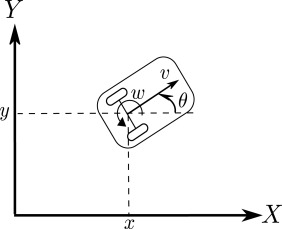
\includegraphics[width=0.5\linewidth]{img/SMC.jpg}
    \caption{Sliding Mode Control}
    \label{fig:SMC}
\end{figure}

